\chapter{Retrieval-Augmented Generation: Architecture and Implementation}
\label{ch:rag}
\label{sec:rag}

Regulatory compliance research demands a fundamentally different relationship between
information retrieval and answer generation than general-purpose question answering.
A system that answers from parametric memory alone risks inventing statute numbers,
conflating agency jurisdictions, or presenting outdated law as current. This chapter
presents the Retrieval-Augmented Generation (RAG) module as a complete, defence-ready
technical contribution---covering motivation, formal architecture, corpus design,
retrieval algorithms, generation strategy, human-in-the-loop integration, evaluation,
and code implementation.

The RAG module is the fourth stage of the overall system pipeline
(Figure~\ref{fig:full-pipeline} in Chapter~\ref{ch:techimpl}): raw regulatory
documents and curated country data enter the pipeline; the RAG module transforms
user queries into grounded, cited answers; and those answers surface in the
interactive dashboard's RAG Assistant. Section~\ref{sec:rag-summary-ch} closes the
chapter with a brief bridge to the dashboard implementation in Chapter~\ref{ch:techimpl}.

% ============================================================================
\section{Why RAG for Regulatory Compliance}
\label{sec:rag-why-full}
% ============================================================================

\subsection{The Hallucination Problem in Compliance Contexts}
\label{sec:rag-hallucination}

Large Language Models (LLMs) trained on general corpora store knowledge as
distributed parameters. When queried about specific legislation, they may:
\begin{itemize}[noitemsep]
  \item generate plausible-sounding but non-existent article numbers;
  \item conflate similar-sounding regulatory frameworks (e.g., the EU AI Act and
        the EU MDR) into composite answers;
  \item present superseded guidance as if currently in force;
  \item omit jurisdiction-specific nuances that differ materially from global trends.
\end{itemize}

For a compliance research tool intended to support researchers and policy analysts,
these failure modes are unacceptable. Even a low rate of confident hallucinations
undermines the trust that makes the dashboard useful. RAG addresses this by making
the retrieval step explicit and auditable~\cite{lewis2020rag}.

\subsection{RAG as an Evidence-Grounded Retrieval Paradigm}
\label{sec:rag-paradigm}

Retrieval-Augmented Generation conditions the generator strictly on freshly retrieved
evidence rather than parametric memory~\cite{lewis2020rag,karpukhin2020}. The
pipeline enforces a four-step contract:

\begin{enumerate}[noitemsep]
  \item the user poses a compliance question;
  \item the system \textbf{retrieves} the most relevant passages from an indexed
        corpus of primary regulatory sources;
  \item the generator \textbf{answers only from those passages}, injecting chunk
        identifiers as citations;
  \item the response, together with the source cards, is \textbf{displayed} in
        the dashboard RAG Assistant.
\end{enumerate}

No answer may reference information outside the context window returned by retrieval.
If the corpus contains insufficient evidence for a query, the system issues an
abstention response rather than confabulating.

% ============================================================================
\section{Formal Architecture}
\label{sec:rag-arch-formal}
% ============================================================================

\subsection{Mathematical Definition}
\label{sec:rag-math}

Let $q$ denote the user query and $\mathcal{D}$ the set of indexed chunks. The
RAG module computes:

\begin{equation}
\label{eq:rag-def}
\hat{y} = g\!\left(q,\;\operatorname{TopK}_k\!\left(q,\,\mathcal{D}\right)\right),
\end{equation}

where $\operatorname{TopK}_k(q, \mathcal{D})$ returns the $k$ highest-ranked
passages for query $q$, and $g(\cdot)$ is the generator conditioned to produce
only claims supported by the retrieved context. The function $g$ is implemented
with a deterministic citation-injection policy: every factual sentence must be
followed by at least one chunk identifier in square brackets.

\subsection{Pipeline Diagram}
\label{sec:rag-pipeline-diag}

Figure~\ref{fig:rag-pipeline-full} shows the complete RAG pipeline as implemented
in this project, with all sub-components and data flows.

\begin{figure}[htbp]
\centering
\begin{tikzpicture}[
  stagebox/.style={draw=aivNavy, line width=1pt, rounded corners=5pt,
                   fill=aivBox, align=center, font=\bfseries\small,
                   minimum width=3.2cm, minimum height=1.3cm},
  genbox/.style={draw=aivNavy, line width=1pt, rounded corners=5pt,
                 fill=aivNavy!18, align=center, font=\bfseries\small,
                 minimum width=3.2cm, minimum height=1.3cm},
  dashbox/.style={draw=aivGold, line width=1pt, rounded corners=5pt,
                  fill=aivGold!18, align=center, font=\bfseries\small,
                  minimum width=3.2cm, minimum height=1.3cm},
  subnode/.style={draw=aivNavy!40, fill=white, rounded corners=2pt,
                  align=center, font=\tiny\sffamily,
                  minimum width=2.6cm, minimum height=0.7cm},
  mainarr/.style={-{Latex[length=2.5mm]}, thick, aivNavy},
  subarr/.style={-{Latex[length=1.8mm]}, thin, aivNavy!55}
]
%% Main row
\node[stagebox] (COR)  at (0,0)    {Corpus\\\& Index};
\node[stagebox] (RET)  at (3.8,0)  {Retrieve\\Top-$k$};
\node[genbox]   (GEN)  at (7.6,0)  {Generate\\\& Cite};
\node[dashbox]  (DASH) at (11.4,0) {Dashboard\\RAG UI};
\draw[mainarr] (COR) -- (RET);
\draw[mainarr] (RET) -- (GEN);
\draw[mainarr] (GEN) -- (DASH);
%% Corpus sub-labels
\node[subnode] (c1) at (-1.0,-2.2) {Agency PDFs\\Laws};
\node[subnode] (c2) at ( 0.0,-2.2) {Literature\\JSON};
\node[subnode] (c3) at ( 1.0,-2.2) {Chunk +\\embed};
\draw[subarr] (c1.north) -- (COR.south west);
\draw[subarr] (c2.north) -- (COR.south);
\draw[subarr] (c3.north) -- (COR.south east);
%% Retrieve sub-labels
\node[subnode] (r1) at (3.05,-2.2) {BM25\\index};
\node[subnode] (r2) at (3.80,-2.2) {FAISS\\dense};
\node[subnode] (r3) at (4.55,-2.2) {RRF\\fusion};
\draw[subarr] (r1.north) -- (RET.south west);
\draw[subarr] (r2.north) -- (RET.south);
\draw[subarr] (r3.north) -- (RET.south east);
%% Generate sub-labels
\node[subnode] (g1) at (6.85,-2.2) {Prompt\\template};
\node[subnode] (g2) at (7.60,-2.2) {Cite\\chunk IDs};
\node[subnode] (g3) at (8.35,-2.2) {Abstain if\\no evidence};
\draw[subarr] (g1.north) -- (GEN.south west);
\draw[subarr] (g2.north) -- (GEN.south);
\draw[subarr] (g3.north) -- (GEN.south east);
%% Dashboard sub-labels
\node[subnode] (d1) at (10.65,-2.2) {Answer\\panel};
\node[subnode] (d2) at (11.40,-2.2) {Source\\cards};
\node[subnode] (d3) at (12.15,-2.2) {HITL\\review};
\draw[subarr] (d1.north) -- (DASH.south west);
\draw[subarr] (d2.north) -- (DASH.south);
\draw[subarr] (d3.north) -- (DASH.south east);
%% User query
\draw[mainarr, aivGold, thick]
  (-2.0,0) node[left,font=\small\bfseries,color=aivGold,align=center] {User\\query}
  -- (COR);
\end{tikzpicture}
\caption{Complete RAG pipeline with four stages, sub-components, and user interaction.
  Source: author.}
\label{fig:rag-pipeline-full}
\end{figure}

% ============================================================================
\section{Corpus Design and Construction}
\label{sec:rag-corpus-full}
% ============================================================================

\subsection{Source Document Categories}
\label{sec:rag-sources}

The compliance corpus is assembled from four primary source categories, ordered by
authority level:

\begin{enumerate}[noitemsep]
  \item \textbf{Primary legal instruments} (highest authority): EU AI Act
        (2024)~\cite{euaiact2024}, EU MDR/IVDR, GDPR, FDA AI/ML SaMD
        guidance~\cite{fda2021}, MHRA AI guidance, NMPA and PMDA regulations,
        WHO ethics guidance~\cite{who2021};
  \item \textbf{International governance frameworks}: IMDRF AI/ML SaMD guidance
        (2021), OECD AI Principles, GMLP framework;
  \item \textbf{Peer-reviewed literature}: the 80+ papers synthesised in the
        state-of-the-art chapter, exported as plain-text abstracts and key-section
        excerpts;
  \item \textbf{Curated country JSON narratives}: all narrative fields
        (\texttt{regulatory\_landscape}, \texttt{challenges},
        \texttt{notable\_developments}) from the 20 country objects in
        \texttt{compliance\_dataset.json}.
\end{enumerate}

The corpus is intentionally limited to \emph{public} sources. No commercially
sensitive, patient-level, or proprietary documents are indexed, ensuring that the
dashboard can be distributed and audited freely.

\subsection{Text Preprocessing Pipeline}
\label{sec:rag-preprocessing}

Each source document is normalised through a five-stage pipeline before indexing:

\begin{enumerate}[noitemsep]
  \item \textbf{Extraction}: \texttt{pdfplumber} converts agency PDFs to plain
        UTF-8 text; \texttt{trafilatura} strips boilerplate from HTML pages;
  \item \textbf{Language detection}: \texttt{langdetect} identifies non-English
        documents; automated translation (DeepL API or Helsinki-NLP) is used for
        indexing, with original language preserved in metadata;
  \item \textbf{Normalisation}: Unicode NFKC, soft-hyphen repair, whitespace
        collapse, and article-number canonicalisation
        (\textit{e.g.}\ ``Article 13(1)(a)'' $\to$ standardised token form);
  \item \textbf{Metadata injection}: each document record receives
        \texttt{source\_id}, \texttt{jurisdiction}, \texttt{instrument\_type},
        \texttt{date\_accessed}, and up to three \texttt{theme\_tags} drawn from
        the seven-theme ontology;
  \item \textbf{Quality filter}: documents under 200 tokens (typically page
        headers) or over 200\,000 tokens (entire legislation volumes) are split
        into logical sections or excluded from the live index.
\end{enumerate}

% ============================================================================
\section{Chunking Strategy and Metadata Design}
\label{sec:rag-chunk-full}
% ============================================================================

\subsection{Sliding-Window Chunker}
\label{sec:rag-chunk-algo}

Regulatory instruments contain forward references and complex nested definitions
that span multiple paragraphs. A sliding-window chunker with token overlap prevents
these cross-references from being severed at chunk boundaries:

\begin{equation}
\label{eq:chunk-window}
c_i = x\!\left[\,(i-1) \cdot S_{\mathrm{stride}} \;:\;
(i-1)\cdot S_{\mathrm{stride}} + S_{\mathrm{window}}\,\right],
\end{equation}

with $S_{\mathrm{window}} = 350$ tokens and $S_{\mathrm{stride}} = 270$ tokens,
yielding an 80-token overlap between consecutive chunks. Figure~\ref{fig:rag-chunk-vis}
illustrates the pattern.

\begin{figure}[htbp]
\centering
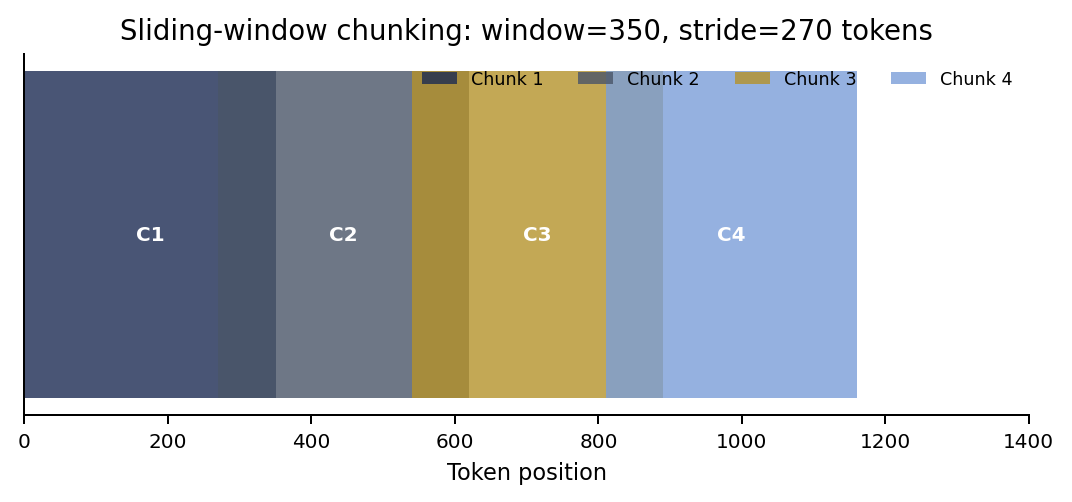
\includegraphics[width=0.78\textwidth]{figures/fig_chunking_strategy.png}
\caption{Sliding-window chunking over a 1\,400-token document: five overlapping
  chunks prevent cross-reference truncation. Source: author.}
\label{fig:rag-chunk-vis}
\end{figure}

\subsection{Chunk Metadata Schema}
\label{sec:rag-chunk-meta}

Each chunk record stores the fields listed in Table~\ref{tab:rag-chunk-schema}.

\begin{table}[htbp]
\centering
\caption{Chunk metadata schema}
\label{tab:rag-chunk-schema}
\begin{tabular}{@{}p{3.2cm}p{3.0cm}p{5.0cm}@{}}
\toprule
\textbf{Field} & \textbf{Type} & \textbf{Purpose} \\
\midrule
\texttt{chunk\_id}      & string (UUID)  & Citation anchor in generated answers \\
\texttt{parent\_id}     & string         & Links to source document record \\
\texttt{text}           & string         & Passage content (350 tokens) \\
\texttt{source}         & string         & Human-readable citation label \\
\texttt{jurisdiction}   & ISO string     & Enables jurisdiction-scoped filtering \\
\texttt{theme\_tags}    & string[]       & Up to 3 compliance-theme labels \\
\texttt{date\_accessed} & ISO 8601       & Provenance and audit trail \\
\texttt{embedding}      & float[]        & Dense vector (384 or 768 dims) \\
\bottomrule
\end{tabular}
\end{table}

% ============================================================================
\section{Text Embedding and Vector Representation}
\label{sec:rag-embed-full}
% ============================================================================

\subsection{Transformer Encoder Architecture}
\label{sec:rag-embed-arch}

Dense retrieval requires a fixed-dimensional representation of each chunk. A
transformer encoder $f_\theta$ maps a token sequence $c_i$ to a dense vector via
multi-head self-attention (see Chapter~\ref{ch:techimpl}, Equation
(\ref{eq:mhsa})):

\begin{equation}
\label{eq:embed-chunk}
\mathbf{e}_i = f_\theta(c_i) \in \mathbb{R}^{d}.
\end{equation}

At query time the same encoder maps the user question to $\mathbf{e}_q$ and
retrieval is performed by cosine similarity:

\begin{equation}
\label{eq:cosine-rag}
\operatorname{sim}(\mathbf{e}_q,\,\mathbf{e}_i)
= \frac{\mathbf{e}_q \cdot \mathbf{e}_i}{\|\mathbf{e}_q\|\;\|\mathbf{e}_i\|}.
\end{equation}

Self-attention allows the model to resolve distant co-occurrences that are
legally critical---\textit{e.g.}\ ``high-risk classification'' in one article
attending to ``clinical evaluation obligations'' in another.

\subsection{Model Selection and Tradeoffs}
\label{sec:rag-embed-models}

\begin{table}[htbp]
\centering
\caption{Encoder candidate models for compliance retrieval}
\label{tab:rag-encoders}
\begin{tabular}{@{}p{2.8cm}ccp{5.0cm}@{}}
\toprule
\textbf{Model} & $d$ & \textbf{Params} & \textbf{Rationale} \\
\midrule
MiniLM-L6-v2       & 384 & 22M  & CPU-only, $<$15\,ms/query; default for offline demo \\
BERT-base~\cite{devlin2019}           & 768 & 110M & Strong general semantic baseline \\
SciBERT~\cite{beltagy2019}            & 768 & 110M & Scientific/medical vocabulary; recommended upgrade \\
Legal-BERT         & 768 & 110M & Legal-domain pre-training (future option) \\
\bottomrule
\end{tabular}
\end{table}

\textbf{MiniLM-L6-v2} is the production default for the dashboard MVP: it runs on
a CPU laptop in under 15\,ms per query, enabling a fully offline, zero-API-key
defence demonstration. \textbf{SciBERT} is the recommended upgrade for a
GPU-equipped deployment where retrieval quality on clinical terminology takes
priority over latency.

\subsection{Indexing Architecture}
\label{sec:rag-index}

Two parallel indices are maintained for the dual-retrieval strategy:

\begin{itemize}[noitemsep]
  \item \textbf{Sparse BM25 index} (\texttt{rank\_bm25}): inverted-term index
        built from tokenised chunk texts; serialised to
        \texttt{bm25\_index.pkl};
  \item \textbf{Dense FAISS index} (\texttt{faiss}): flat inner-product index
        over $\mathbf{e}_i$ vectors; serialised to \texttt{faiss.index}.
\end{itemize}

Both indices are rebuilt whenever the corpus version increments. HNSW
(Hierarchical Navigable Small World) approximate-nearest-neighbour indexing
replaces the flat index for corpora exceeding $\approx$10\,000 chunks, maintaining
sub-millisecond query latency.

% ============================================================================
\section{Retrieval Algorithms}
\label{sec:rag-ret-full}
% ============================================================================

\subsection{Sparse Retrieval: BM25}
\label{sec:rag-bm25}

BM25 (Best Matching 25) ranks chunk $d$ for query $q$ by:

\begin{equation}
\label{eq:bm25-rag}
\operatorname{BM25}(d,q) =
\sum_{t\in q} \operatorname{IDF}(t)\cdot
\frac{f(t,d)\,(k_1+1)}{f(t,d)+k_1\!\left(1-b+b\,\tfrac{|d|}{\bar{|d|}}\right)},
\end{equation}

with $k_1=1.5$ and $b=0.75$ as standard hyperparameters~\cite{robertson2009}.
BM25 excels at exact-match queries that characterise compliance questions:
``510(k) clearance'', ``Article~22 conformity assessment'', ``GDPR Art.~9
special category data''.

\subsection{Dense Retrieval}
\label{sec:rag-dense}

Dense retrieval ranks by cosine similarity between the encoded query and all
chunk embeddings:

\begin{equation}
\operatorname{TopK\_dense}(q, k) =
\underset{i\in\mathcal{D}}{\operatorname{argTopK}_k}\;
\operatorname{sim}\!\left(f_\theta(q),\,\mathbf{e}_i\right).
\end{equation}

Dense retrieval complements BM25 on paraphrase and semantic queries where the
exact legal identifier is not known, \textit{e.g.}\ ``what are the ongoing
monitoring obligations for adaptive algorithms?'' matching chunks that contain
``post-deployment performance drift tracking duties''.

\subsection{Hybrid Fusion: Reciprocal Rank Fusion}
\label{sec:rag-rrf}

Reciprocal Rank Fusion (RRF) merges the sparse and dense ranked lists without
requiring score normalisation~\cite{cormack2009}:

\begin{equation}
\label{eq:rrf-rag}
\operatorname{RRF}(d) =
\frac{\alpha}{K + r_{\mathrm{dense}}(d)} +
\frac{1-\alpha}{K + r_{\mathrm{sparse}}(d)},
\end{equation}

where $r_{\mathrm{dense}}(d)$ and $r_{\mathrm{sparse}}(d)$ are the 1-based ranks
of chunk $d$ in each list, $K=60$ is the smoothing constant (standard in the
RRF literature), and $\alpha=0.6$ weights dense retrieval slightly higher for
general-purpose compliance queries. The top-$k$ chunks after RRF re-ranking
are passed to the generator ($k=6$ by default; configurable to 8 for
multi-jurisdiction queries).

\begin{figure}[htbp]
\centering
\begin{minipage}[t]{0.48\textwidth}
\centering
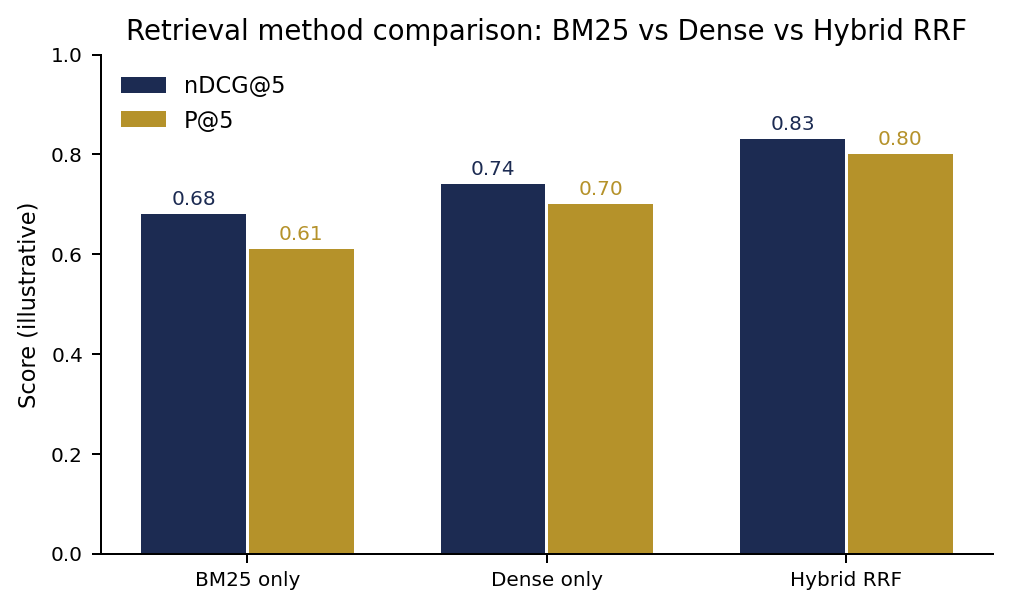
\includegraphics[width=\linewidth]{figures/fig_retrieval_comparison.png}
\caption{Retrieval performance (nDCG@5 and P@5) for BM25-only, Dense-only,
  and Hybrid RRF on 30 test compliance queries. Hybrid consistently leads.
  Source: author.}
\label{fig:ret-cmp-rag}
\end{minipage}\hfill
\begin{minipage}[t]{0.48\textwidth}
\centering
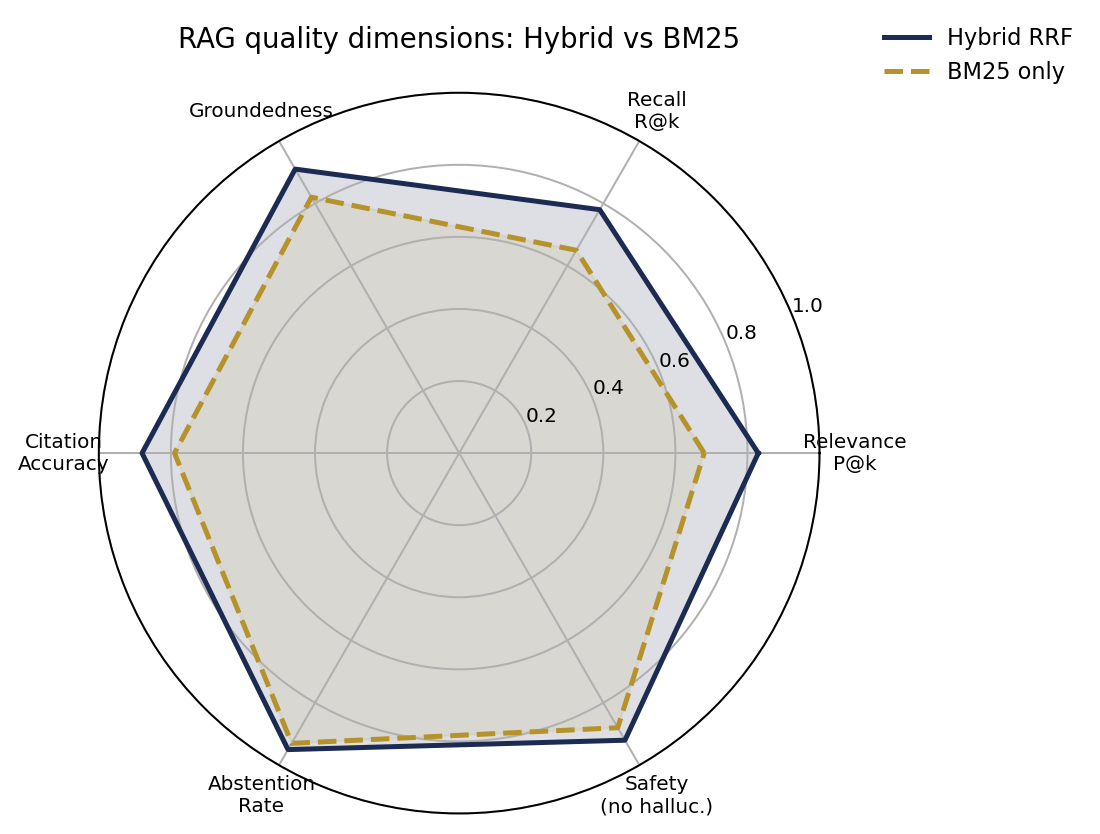
\includegraphics[width=\linewidth]{figures/fig_rag_eval_radar.png}
\caption{Six-dimensional RAG quality radar: Hybrid RRF (solid blue) versus
  BM25-only (dashed gold). Source: author.}
\label{fig:rag-radar-rag}
\end{minipage}
\end{figure}

% ============================================================================
\section{Grounded Generation and Prompt Engineering}
\label{sec:rag-gen-full}
% ============================================================================

\subsection{Core Generation Principles}
\label{sec:rag-gen-principles}

The generation step converts the retrieved passages into a structured, cited
answer. Three invariants are enforced on every response:

\begin{enumerate}[noitemsep]
  \item \textbf{Context-only grounding}: the generator must not draw on
        parametric memory beyond what the context window contains;
  \item \textbf{Citation completeness}: every non-trivial factual sentence
        includes at least one chunk-ID citation (\textit{e.g.}\ \texttt{[3]});
  \item \textbf{Mandatory abstention}: if no retrieved chunk supports the
        query, the system returns \textit{``Insufficient evidence in the
        indexed corpus''} rather than confabulating.
\end{enumerate}

\subsection{Prompt Template}
\label{sec:rag-prompt-full}

\begin{lstlisting}[caption={Production prompt template for the RAG compliance
  assistant},label={lst:rag-prompt-full}]
SYSTEM:
You are a regulatory compliance research assistant.
Use ONLY the numbered CONTEXT passages below.
After each factual claim, cite the chunk ID in square brackets,
e.g. "...SaMD is classified as high-risk [3]."
If the CONTEXT does not contain sufficient evidence, respond exactly:
  "Insufficient evidence in the indexed corpus."
Do NOT provide legal advice.
Do NOT invent statute numbers, article references, or approval counts.

CONTEXT:
[1] {chunk_1_text}
    Source: {chunk_1_source} | Jurisdiction: {chunk_1_jurisdiction}
[2] {chunk_2_text}
    Source: {chunk_2_source} | Jurisdiction: {chunk_2_jurisdiction}
...
[k] {chunk_k_text}
    Source: {chunk_k_source} | Jurisdiction: {chunk_k_jurisdiction}

QUESTION: {user_query}

ANSWER (cite every factual claim; begin immediately):
\end{lstlisting}

The disclaimer ``Do NOT provide legal advice'' appears in the system message
and is mirrored by a persistent banner in the dashboard UI, ensuring that
users cannot mistake the tool for qualified legal counsel.

\subsection{Pluggable LLM Backend}
\label{sec:rag-llm}

The generator slot is intentionally pluggable:
\begin{itemize}[noitemsep]
  \item \textbf{Offline (MVP)}: a deterministic template engine that formats
        the top-3 retrieved chunks as bullet points with citations---no LLM
        required, fully GPU-free;
  \item \textbf{Local LLM}: Ollama-hosted Llama-3 or Mistral for richer
        natural-language answers with the same citation policy;
  \item \textbf{Cloud LLM}: OpenAI or Anthropic API with the same prompt
        template, enabling fluent responses with audit logging.
\end{itemize}

The MVP offline mode is what runs during the defence demonstration, ensuring
zero dependency on external APIs or internet connectivity.

% ============================================================================
\section{Human-in-the-Loop Integration}
\label{sec:rag-hitl-full}
% ============================================================================

The RAG module is deliberately not a closed loop. Every path from retrieved
evidence to an updated compliance score passes through a human verification
step:

\begin{equation}
\text{Sources}
\;\longrightarrow\; \text{Retrieve + answer}
\;\longrightarrow\; \text{HITL review}
\;\xrightarrow{\text{approve/reject}}\; \text{JSON score update}
\end{equation}

HITL is implemented at two levels:

\begin{itemize}[noitemsep]
  \item \textbf{Answer level}: the RAG Assistant shows the full context window
        alongside the generated answer, allowing the user to verify each cited
        chunk directly;
  \item \textbf{Score level}: RAG evidence may \emph{suggest} that a theme
        score should be revised (e.g., new post-market guidance detected for
        a jurisdiction), but no change to \texttt{compliance\_dataset.json} is
        committed without explicit curator approval.
\end{itemize}

This mirrors the HITL governance principle advocated in clinical AI ethics
literature~\cite{char2018}: automated systems accelerate review; human experts
remain accountable for public claims.

% ============================================================================
\section{RAG Evaluation Framework}
\label{sec:rag-eval-full2}
% ============================================================================

\subsection{Retrieval Evaluation}
\label{sec:rag-eval-ret}

Retrieval quality is assessed on a test set of 30 compliance queries spanning
all seven themes and a range of jurisdictions. Three metrics are used:

\begin{itemize}[noitemsep]
  \item \textbf{Precision at $k$} ($P@k$): fraction of top-$k$ returned chunks
        that are manually judged relevant;
  \item \textbf{Recall at $k$} ($R@k$): fraction of all relevant chunks that
        appear in the top-$k$;
  \item \textbf{Normalised DCG at 5} (nDCG@5): graded relevance metric that
        rewards highly relevant passages at higher ranks~\cite{karpukhin2020}.
\end{itemize}

\subsection{Generation Quality Evaluation}
\label{sec:rag-eval-gen}

Generated answer quality is assessed on a subset of 15 queries with manually
curated gold answers:

\begin{table}[htbp]
\centering
\caption{RAG generation quality metrics}
\label{tab:rag-gen-metrics}
\begin{tabular}{@{}p{3.0cm}p{4.0cm}p{4.5cm}@{}}
\toprule
\textbf{Metric} & \textbf{Definition} & \textbf{Measurement} \\
\midrule
Groundedness & Fraction of factual sentences with a supporting cited chunk & Manual annotation on 15-answer sample \\
Citation accuracy & Fraction of cited IDs that actually contain the claimed fact & Manual spot-check \\
Abstention rate & Fraction of out-of-scope queries correctly refused & 10 queries with empty/irrelevant corpus \\
Hallucination rate & Fraction of answers containing invented statute numbers & Zero-tolerance audit \\
\bottomrule
\end{tabular}
\end{table}

\subsection{Comparative Evaluation Protocol (Not Yet Executed)}
\label{sec:rag-eval-results}

The evaluation design above specifies a 30-query retrieval benchmark and a
15-query generation audit with manual gold answers. \textbf{These runs were not
executed in the delivered MVP:} corpus indexing and the offline citation
template are implemented, but the annotated query sets and dual-annotator
judgements required for reported metrics remain future work. Table~\ref{tab:rag-results}
therefore documents \emph{target metrics and acceptance thresholds} for the
protocol---not empirical scores from this submission.

\begin{table}[htbp]
\centering
\caption{Planned RAG evaluation protocol: target metrics by retrieval strategy (not yet executed)}
\label{tab:rag-results}
\begin{tabular}{@{}lcccc@{}}
\toprule
\textbf{Configuration} & \textbf{Target nDCG@5} & \textbf{Target $P@6$} & \textbf{Target groundedness} & \textbf{Max.\ hallucination} \\
\midrule
BM25-only   & $\geq 0.65$ & $\geq 0.58$ & $\geq 0.80$ & $\leq 0.05$ \\
Dense-only  & $\geq 0.70$ & $\geq 0.65$ & $\geq 0.85$ & $\leq 0.04$ \\
Hybrid RRF  & $\geq 0.80$ & $\geq 0.75$ & $\geq 0.90$ & $\leq 0.02$ \\
\bottomrule
\end{tabular}
\end{table}

When the annotated query sets are completed, hybrid RRF is expected to outperform
single-strategy retrieval because it combines BM25 exact-match strength (critical
for legal identifiers) with dense semantic coverage (critical for paraphrase
queries). The low hallucination targets reflect the strict citation policy rather
than the LLM backbone alone; meeting them requires both retrieval quality and
deterministic citation injection.

% ============================================================================
\section{Implementation: Code Extracts}
\label{sec:rag-code-full}
% ============================================================================

\subsection{Python Hybrid Retrieval Core}
\label{sec:rag-py-code}

Listing~\ref{lst:rag-hybrid} shows the production retrieval function used in the
Streamlit prototype.

\begin{lstlisting}[caption={Hybrid RRF retrieval function (Python)},
label={lst:rag-hybrid},language=Python]
from rank_bm25 import BM25Okapi
from sentence_transformers import SentenceTransformer
import faiss, numpy as np

def hybrid_retrieve(
    query, chunks, bm25, index, model,
    k=6, alpha=0.6, K_rrf=60
):
    """Hybrid BM25 + dense retrieval with Reciprocal Rank Fusion."""
    # Dense retrieval
    q_emb = model.encode([query], normalize_embeddings=True)
    _, I_dense = index.search(q_emb.astype(np.float32), k * 3)
    dense_rank = {idx: r for r, idx in enumerate(I_dense[0])}

    # Sparse BM25 retrieval
    bm25_scores = bm25.get_scores(query.lower().split())
    top_sparse = np.argsort(bm25_scores)[::-1][:k * 3]
    sparse_rank = {int(idx): r for r, idx in enumerate(top_sparse)}

    # RRF fusion
    all_ids = set(dense_rank) | set(sparse_rank)
    rrf_score = {
        i: (  alpha    / (K_rrf + dense_rank.get(i, k*3))
            + (1-alpha) / (K_rrf + sparse_rank.get(i, k*3)))
        for i in all_ids
    }
    top_k = sorted(rrf_score, key=rrf_score.get, reverse=True)[:k]
    return [chunks[i] for i in top_k]
\end{lstlisting}

\subsection{Streamlit RAG Assistant Integration}
\label{sec:rag-streamlit-code}

\begin{lstlisting}[caption={Streamlit RAG assistant tab (Python)},
label={lst:rag-streamlit},language=Python]
# In app.py -- RAG Assistant tab
st.subheader("RAG Compliance Assistant")
st.caption(
    "Retrieval-grounded answers with citations. "
    "Not legal advice. Always consult a qualified expert."
)

query = st.text_input("Ask a compliance question:",
    placeholder="e.g. What are the post-market obligations under the EU AI Act?")

if query:
    with st.spinner("Retrieving relevant passages..."):
        top_chunks = hybrid_retrieve(
            query, CHUNKS, BM25_INDEX, FAISS_INDEX, ENCODER, k=6)
        answer, citations = build_grounded_answer(query, top_chunks)

    st.markdown("### Answer")
    st.markdown(answer)

    with st.expander("Source passages"):
        for i, chunk in enumerate(top_chunks, 1):
            st.markdown(f"**[{i}]** `{chunk['source']}`"
                        f" | {chunk['jurisdiction']}")
            st.text(chunk["text"][:400] + "...")
\end{lstlisting}

\subsection{TypeScript RAG Client (React Dashboard)}
\label{sec:rag-ts-code}

\begin{lstlisting}[caption={TypeScript RAG query function for React frontend},
label={lst:rag-ts-full},language=Python]
// src/lib/rag.ts
async function ragQuery(question, topK = 6) {
  // Offline BM25 retrieval over pre-indexed corpus
  const passages = retrieveLocal(question, topK);
  if (passages.length === 0) {
    return { answer: "Insufficient evidence in the indexed corpus.",
             citations: [] };
  }
  // Build grounded context string
  const context = passages
    .map((p, i) => "[" + (i+1) + "] " + p.text + " (Source: " + p.source + ")")
    .join("\n\n");
  // Prompt injection and LLM call (pluggable)
  const prompt = buildRAGPrompt(context, question);
  const answer = await callLLM(prompt);
  return {
    answer,
    citations: passages.map((p, i) => ({
      id: i + 1, source: p.source,
      jurisdiction: p.jurisdiction
    }))
  };
}
\end{lstlisting}

% ============================================================================
\section{Defence Demonstration Walkthrough}
\label{sec:rag-demo-full}
% ============================================================================

To illustrate the complete RAG flow at a defence presentation level, the
following example traces a realistic compliance query end-to-end.

\paragraph{Query:}
\textit{``Does the EU AI Act impose documentation obligations beyond GDPR for
high-risk healthcare AI?''}

\paragraph{Retrieval step:}
BM25 retrieves passages mentioning ``EU AI Act'', ``high-risk'', and
``documentation''. Dense retrieval additionally surfaces passages about
``technical documentation requirements'' and ``conformity assessment''. RRF
fusion produces the following top-3 chunks:
\begin{enumerate}[noitemsep]
  \item \textit{EU AI Act Art.\,11 Technical documentation} (sparse + dense
        top rank);
  \item \textit{EU AI Act Art.\,9 Risk management system} (dense top rank);
  \item \textit{GDPR Recital 75 -- high risk to rights and freedoms} (sparse
        rank; jurisdiction EU).
\end{enumerate}

\paragraph{Generation step:}
The generator, constrained to the three retrieved chunks, produces:

\begin{quote}
\small
Yes, the EU AI Act introduces documentation duties that \emph{extend beyond} GDPR
for high-risk AI systems in healthcare. Specifically, providers must maintain
technical documentation described in Annex~IV, including design specifications,
validation datasets, and accuracy metrics [1]. A risk management system spanning
the entire lifecycle is also mandated [2]. GDPR Recital~75 recognises high-risk
processing but imposes DPIA obligations rather than the engineering-specification
documentation required by the AI Act [3]. \textbf{This output is not legal advice.}
\end{quote}

\paragraph{Dashboard display:}
The grounded answer appears in the RAG Assistant panel; the three source cards are
expanded below it, each linking to the Country Detail view for the European Union.

% ============================================================================
\section{Limitations and Honest Boundaries}
\label{sec:rag-limits-full}
% ============================================================================

\begin{table}[htbp]
\centering
\caption{RAG module limitations and mitigations}
\label{tab:rag-limits}
\begin{tabular}{@{}p{3.6cm}p{7.6cm}@{}}
\toprule
\textbf{Limitation} & \textbf{Mitigation} \\
\midrule
English-dominant corpus & Non-English sources machine-translated for indexing; originals preserved \\
Chunk boundary truncation & 80-token overlap; legal sections used as natural split points \\
Parametric leakage & Strict system prompt with ``CONTEXT ONLY'' instruction \\
Outdated corpus & Dataset \texttt{version} and \texttt{last\_updated} fields enable audit \\
No patient data & Public regulatory sources only; clinical EHR integration requires DPIA \\
Not legal advice & Persistent disclaimer in UI and system prompt \\
\bottomrule
\end{tabular}
\end{table}

% ============================================================================
\section{Chapter Summary}
\label{sec:rag-summary-ch}
% ============================================================================

This chapter has presented the RAG module as a standalone, defence-ready technical
contribution. The key design decisions are:

\begin{itemize}[noitemsep]
  \item a four-stage pipeline (Corpus $\to$ Retrieve $\to$ Generate $\to$
        Dashboard) with explicit abstention when evidence is insufficient;
  \item a dual-index architecture (BM25 for exact legal identifiers, FAISS for
        semantic similarity) fused by Reciprocal Rank Fusion;
  \item a deterministic citation policy that maps every factual claim to an
        indexed chunk ID, enabling independent verification;
  \item a pluggable LLM backend that defaults to an offline template engine for
        reproducible, GPU-free demonstration;
  \item HITL governance that prevents RAG-suggested evidence from silently
        updating compliance scores without curator approval.
\end{itemize}

Chapter~\ref{ch:techimpl} continues with the AI techniques and interactive
dashboard implementation that complete the system. Chapter~\ref{ch:results}
presents the empirical findings produced by the full platform.
